\section{Analyse globale des cas d'utilisation}

\subsection{Diagramme global}

Le diagramme global de la figure~\ref{fig:global-use-cases} regroupe les capacités
communes et les fonctions propres à chaque rôle. Il distingue les acteurs humains,
la borne de recharge et le service de paiement, puis explicite les dépendances
\texttt{include}, l'extension liée à l'assignation d'une intervention et les
généralisations d'acteurs. Les scénarios détaillés complètent cette vue en précisant
les préconditions, les contrôles d'autorisation et les cas d'erreur.

\begin{landscape}
  \begin{figure}[p]
    \centering
    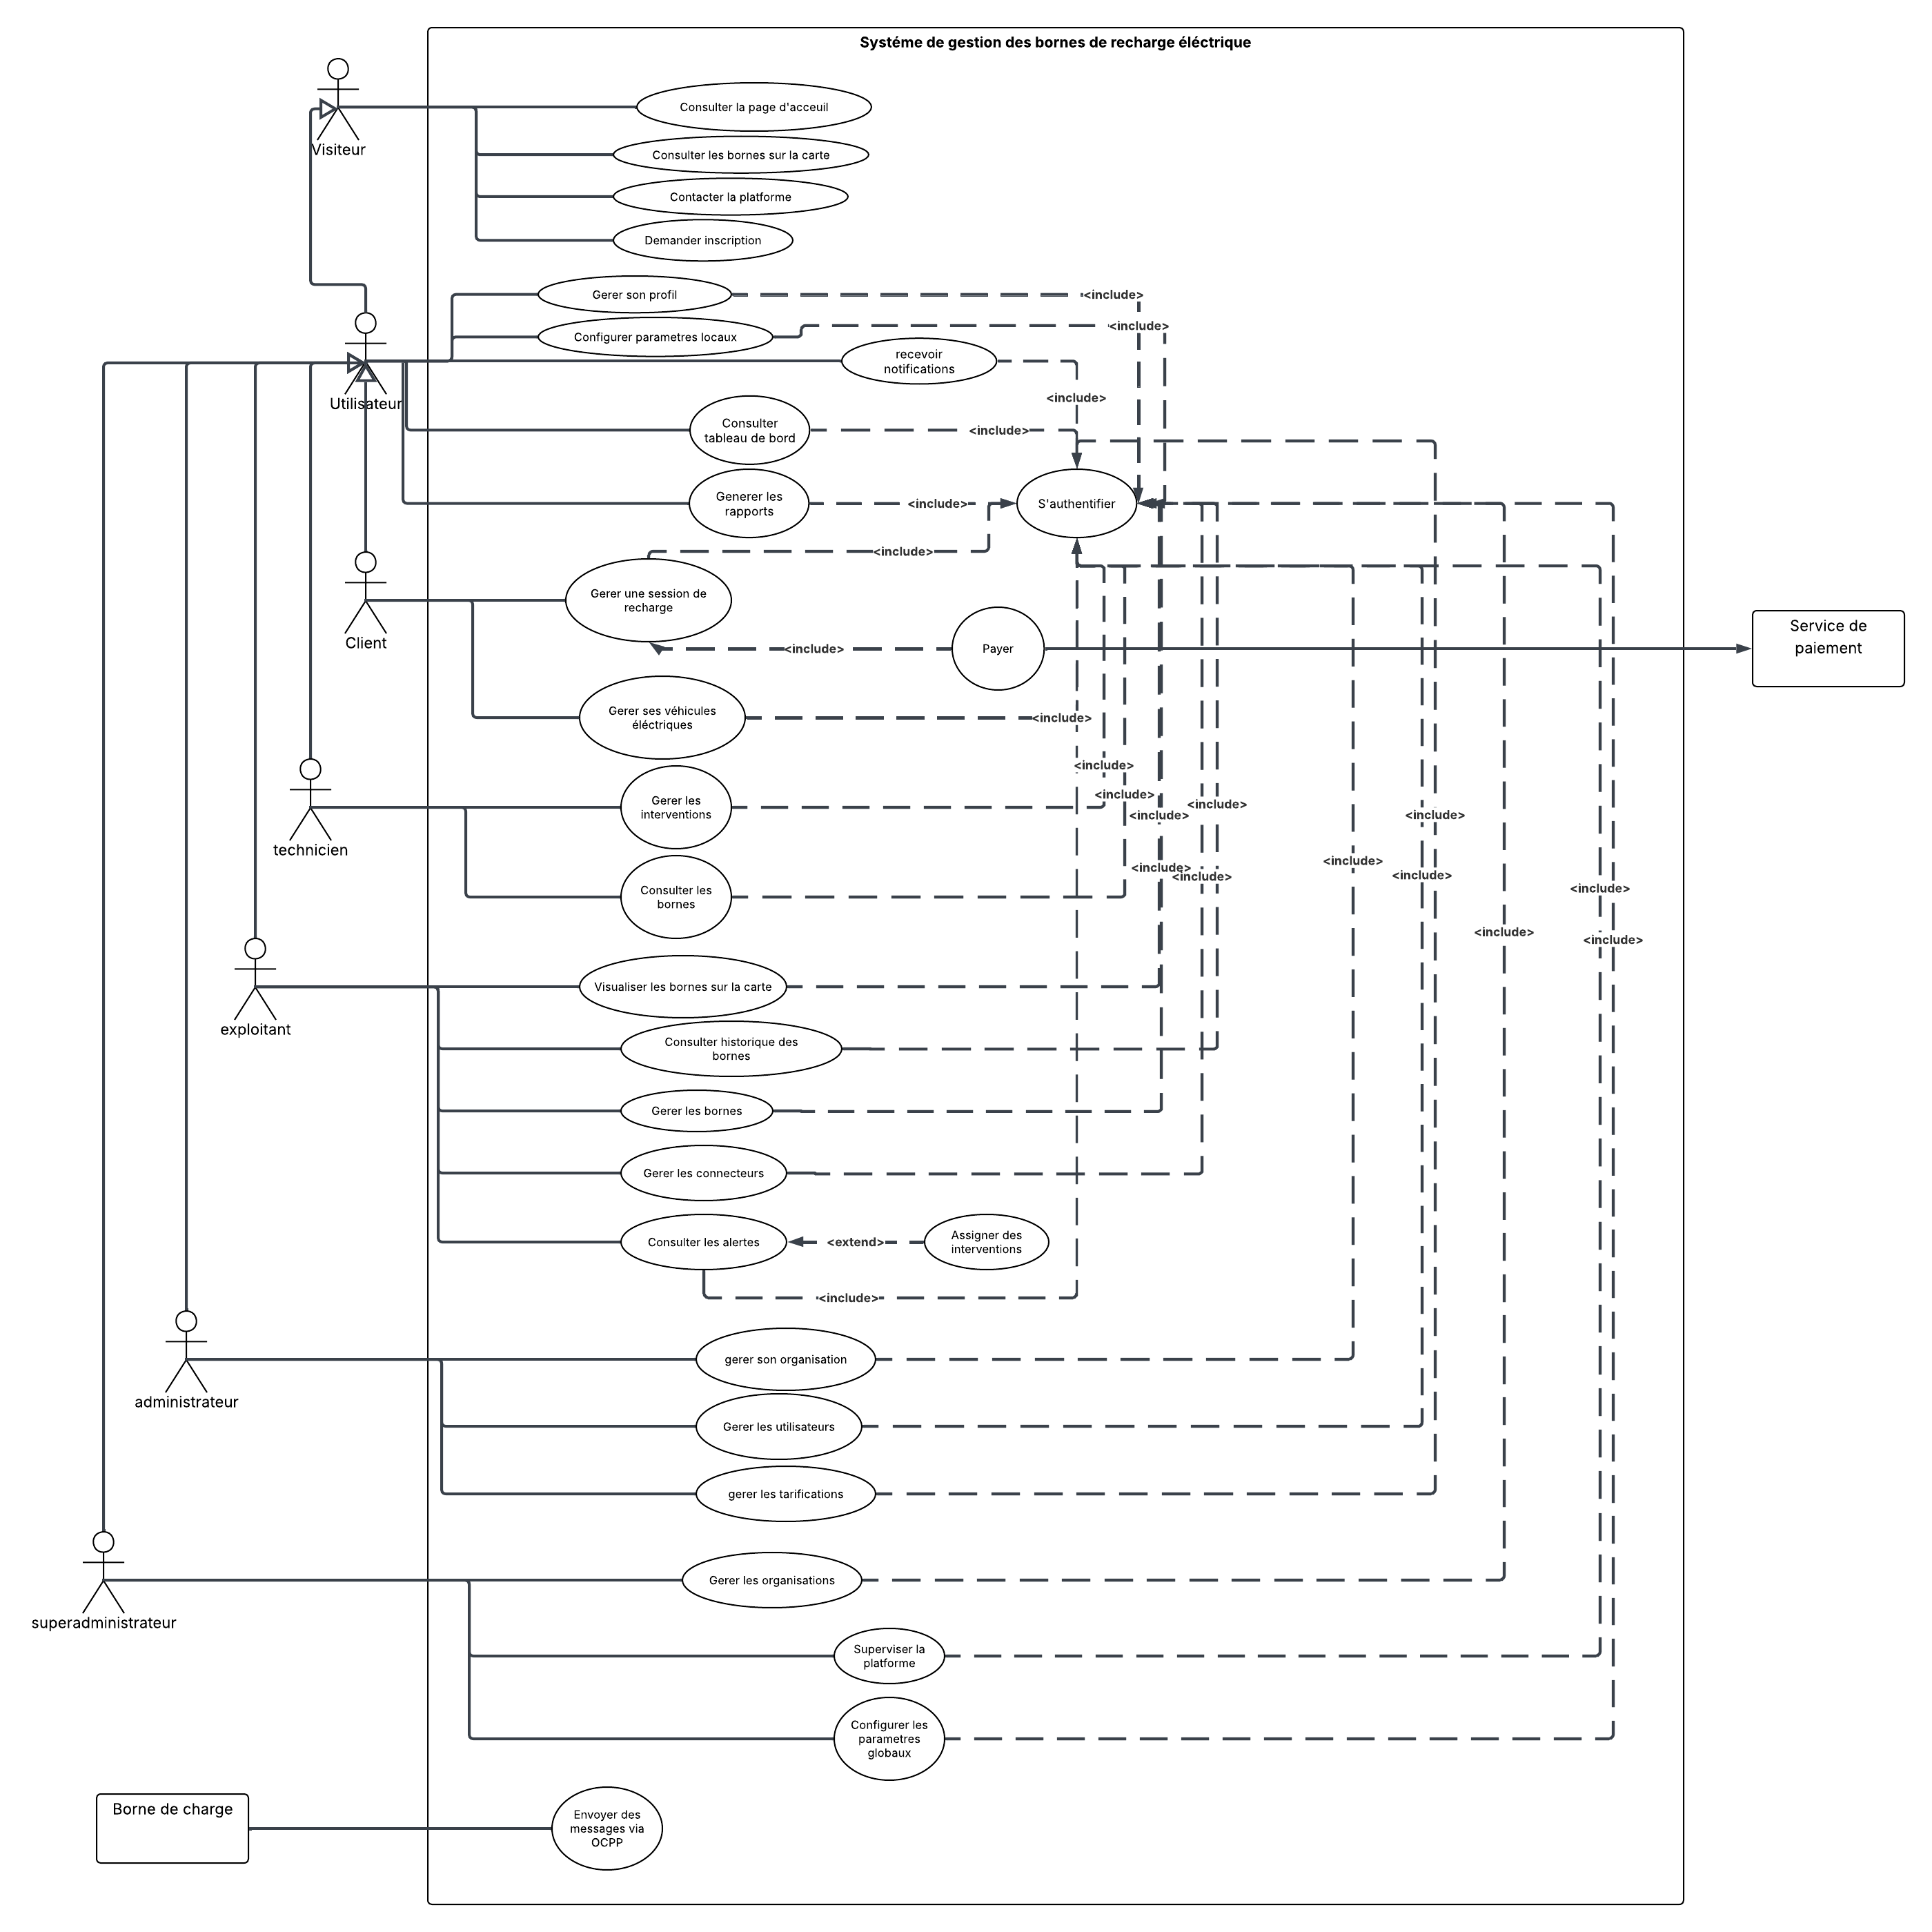
\includegraphics[
      width=0.95\linewidth,
      height=0.82\textheight,
      keepaspectratio
    ]{assets/diagrams/global-use-cases.png}
    \caption{Diagramme global des cas d'utilisation de \ProjectName{}}
    \label{fig:global-use-cases}
  \end{figure}
\end{landscape}

\begin{scopebox}[Conventions du diagramme]
  Les acteurs humains sont représentés par des silhouettes, les systèmes externes
  par des rectangles et les fonctionnalités par des ellipses placées dans la
  frontière du système. Une ligne continue exprime une association ; une flèche en
  pointillés précise une relation \texttt{include} ou \texttt{extend}. Les contrôles
  de permission, l'organisation et les scénarios d'erreur sont détaillés ci-dessous.
\end{scopebox}

\subsection{Catalogue des cas majeurs}

\begin{longtable}{@{}C{1.35cm}p{4.0cm}p{3.3cm}p{5.3cm}@{}}
  \caption{Catalogue des cas d'utilisation majeurs}
  \label{tab:use-case-catalog}\\
  \toprule
  \textbf{ID} & \textbf{Cas d'utilisation} & \textbf{Acteur principal} &
  \textbf{Résultat métier}\\
  \midrule
  \endfirsthead
  \toprule
  \textbf{ID} & \textbf{Cas d'utilisation} & \textbf{Acteur principal} &
  \textbf{Résultat métier}\\
  \midrule
  \endhead
  UC-01 & Demander une démonstration et provisionner une organisation &
  Visiteur, Super Administrateur &
  Une organisation d'essai et son administrateur invité sont créés après décision
  explicite.\\
  UC-02 & Inviter et activer un employé &
  Administrateur &
  Un opérateur ou technicien définit lui-même son mot de passe et rejoint la bonne
  organisation.\\
  UC-03 & Mettre en service une station OCPP &
  Opérateur &
  La station, ses connecteurs et son identité OCPP sont créés atomiquement et prêts à
  être reliés au simulateur ou au matériel.\\
  UC-04 & Calculer la disponibilité &
  Borne / plateforme &
  Les preuves OCPP deviennent un état métier, une transition et, si nécessaire, une
  alerte.\\
  UC-05 & Effectuer une recharge et payer &
  Client &
  Une transaction technique produit une session mesurée, un paiement réconcilié et
  un reçu.\\
  UC-06 & Traiter une alerte et une intervention &
  Opérateur, Technicien &
  L'incident est qualifié, assigné, documenté et clôturé avec une chronologie.\\
  UC-07 & Gérer le cycle commercial d'une organisation &
  Super Administrateur, Administrateur &
  L'essai, l'offre, les limites et factures évoluent sans supprimer les données de
  l'organisation.\\
  UC-08 & Générer et échanger un rapport &
  Utilisateur autorisé &
  Une analyse adaptée au rôle est exportée ou envoyée avec pièces jointes et suivi.\\
  \bottomrule
\end{longtable}

\subsection{UC-01 -- Demander une démonstration et provisionner une organisation}

\begin{table}[H]
  \centering
  \begin{tabularx}{\textwidth}{@{}C{3.3cm}Y@{}}
    \toprule
    \textbf{Objectif} & Convertir une demande publique qualifiée en organisation
    d'essai et compte administrateur sécurisé.\\
    \textbf{Acteurs} & Visiteur et Super Administrateur ; service email comme acteur
    secondaire.\\
    \textbf{Préconditions} & Les demandes de démonstration sont activées ; l'adresse
    n'est pas bloquée par les protections anti-abus.\\
    \textbf{Déclencheur} & Le visiteur valide le formulaire public.\\
    \textbf{Postconditions} & La demande est rejetée ou reliée à une organisation
    d'essai et à une invitation administrateur traçable.\\
    \bottomrule
  \end{tabularx}
\end{table}

\textbf{Scénario nominal}
\begin{enumerate}[leftmargin=8mm]
  \item Le visiteur renseigne son identité, son organisation, sa taille, ses objectifs
  multiples, son message et son consentement.
  \item Le système valide les champs, le honeypot et la limitation de débit, puis
  enregistre la demande au statut \emph{nouvelle}.
  \item Un accusé de réception est envoyé sans lien vers l'espace Super Administrateur.
  \item Le Super Administrateur ouvre la demande et démarre sa revue.
  \item Il vérifie le contexte, ajuste la durée d'essai et saisit le nom de
  l'organisation et de son futur administrateur.
  \item Le système crée atomiquement l'organisation, l'abonnement d'essai, le compte
  administrateur en attente et l'invitation.
  \item L'invitation à usage unique est envoyée au demandeur.
  \item Le demandeur l'accepte, définit son mot de passe, complète éventuellement le
  logo de l'organisation et accède à l'onboarding administrateur.
\end{enumerate}

\textbf{Alternatives et exceptions}
\begin{itemize}[leftmargin=7mm]
  \item si la demande n'est pas pertinente, le Super Administrateur la rejette avec
  une raison ; aucun compte n'est créé ;
  \item si l'email ou l'organisation provoque un conflit, la transaction est annulée
  sans création partielle ;
  \item si l'invitation expire ou doit être invalidée, elle est révoquée avant qu'une
  nouvelle invitation ne soit émise ;
  \item les transitions intermédiaires sans action métier ne sont pas exposées comme
  des statuts sélectionnables manuellement.
\end{itemize}

\subsection{UC-02 -- Inviter et activer un employé}

\begin{table}[H]
  \centering
  \begin{tabularx}{\textwidth}{@{}C{3.3cm}Y@{}}
    \toprule
    \textbf{Objectif} & Donner un accès opérateur ou technicien sans transmettre de
    mot de passe initial.\\
    \textbf{Acteurs} & Administrateur, employé invité et service email.\\
    \textbf{Préconditions} & L'administrateur et son organisation sont actifs ; la
    limite d'employés de l'offre commerciale n'est pas atteinte.\\
    \textbf{Déclencheur} & L'administrateur choisit \emph{Ajouter un employé}.\\
    \textbf{Postconditions} & Le compte activé appartient à exactement une
    organisation et possède uniquement le rôle choisi.\\
    \bottomrule
  \end{tabularx}
\end{table}

\textbf{Scénario nominal}
\begin{enumerate}[leftmargin=8mm]
  \item L'administrateur saisit le nom, l'email, le rôle opérateur ou technicien,
  l'équipe et les coordonnées utiles.
  \item Le backend ignore tout identifiant d'organisation venant du navigateur et
  impose celle de l'administrateur.
  \item Un compte \emph{pending} sans mot de passe utilisable est créé avec une
  invitation limitée dans le temps.
  \item L'employé reçoit le lien, vérifie les informations non modifiables et choisit
  son mot de passe.
  \item L'invitation est consommée une seule fois, le compte devient actif et
  l'onboarding du rôle est proposé à la première connexion.
\end{enumerate}

\textbf{Alternatives et exceptions}
\begin{itemize}[leftmargin=7mm]
  \item un rôle administrateur, client ou super administrateur est refusé dans ce
  workflow ;
  \item un email déjà actif, un quota atteint ou une organisation inactive empêche
  l'invitation ;
  \item l'administrateur peut envoyer un rappel tant que le lien est valide, ou
  renouveler le lien après invalidation de l'ancien ;
  \item aucun administrateur ne peut afficher, choisir ou réinitialiser le mot de
  passe de l'employé.
\end{itemize}

\subsection{UC-03 -- Mettre en service une station OCPP}

\begin{table}[H]
  \centering
  \begin{tabularx}{\textwidth}{@{}C{3.3cm}Y@{}}
    \toprule
    \textbf{Objectif} & Créer une station exploitable, ses connecteurs physiques et
    son identité de communication dans une seule opération.\\
    \textbf{Acteurs} & Opérateur ou Administrateur ; borne physique ou simulateur SAP.\\
    \textbf{Préconditions} & L'organisation est autorisée à ajouter une station et
    n'a pas atteint sa capacité commerciale.\\
    \textbf{Déclencheur} & L'utilisateur ouvre l'assistant de mise en service.\\
    \textbf{Postconditions} & La station est persistée avec ses connecteurs et une
    cible de commissioning ; son secret en clair n'est affiché qu'une fois si requis.\\
    \bottomrule
  \end{tabularx}
\end{table}

\textbf{Scénario nominal}
\begin{enumerate}[leftmargin=8mm]
  \item L'opérateur renseigne le nom, la référence, le fabricant, le modèle, la
  puissance, l'adresse et la version OCPP.
  \item Il clique sur la carte ou déplace le marqueur ; latitude et longitude sont
  remplies automatiquement mais restent éditables.
  \item Il ajoute chaque connecteur avec son libellé, son identifiant OCPP, son type,
  son courant et sa puissance maximale.
  \item Il choisit la cible \emph{simulateur SAP local} ou \emph{station externe} et
  confirme l'identité OCPP.
  \item Le système vérifie les références, identités et identifiants connecteur, puis
  crée l'ensemble dans une transaction.
  \item Pour le simulateur local, l'interface fournit la commande d'enregistrement du
  profil ; pour une borne externe, elle affiche une fois les informations de
  connexion nécessaires.
  \item La borne ouvre sa connexion, envoie \texttt{BootNotification} et
  \texttt{StatusNotification}, puis la fiche reflète la connexion réelle.
\end{enumerate}

\textbf{Alternatives et exceptions}
\begin{itemize}[leftmargin=7mm]
  \item une référence comme \texttt{CT-TUN-001} déjà utilisée doit être remplacée par
  une valeur unique ; elle ne peut pas désigner deux stations ;
  \item une erreur sur un connecteur annule la création complète ;
  \item tant que le simulateur n'est pas enregistré et redémarré, la station reste en
  attente de connexion ; la création en base ne simule pas un heartbeat ;
  \item une rotation de secret invalide l'ancien secret sans modifier l'identité
  publique de la station.
\end{itemize}

\subsection{UC-04 -- Calculer la disponibilité}

\begin{table}[H]
  \centering
  \begin{tabularx}{\textwidth}{@{}C{3.3cm}Y@{}}
    \toprule
    \textbf{Objectif} & Transformer les preuves OCPP et les dérogations autorisées en
    état métier explicable.\\
    \textbf{Acteurs} & Borne ou simulateur ; moteur de projection de la plateforme.\\
    \textbf{Préconditions} & La station est provisionnée pour OCPP et ses connecteurs
    sont connus.\\
    \textbf{Déclencheur} & Connexion, fermeture, message OCPP ou contrôle périodique
    de connectivité.\\
    \textbf{Postconditions} & Les états courants, transitions, alertes et diffusions
    temps réel sont cohérents et audités.\\
    \bottomrule
  \end{tabularx}
\end{table}

\textbf{Scénario nominal}
\begin{enumerate}[leftmargin=8mm]
  \item La passerelle authentifie la station et vérifie la signature de l'appel
  interne transmis à Laravel.
  \item Le message est dédupliqué et persisté avant projection.
  \item Le moteur applique l'ordre : désactivation manuelle, maintenance planifiée,
  perte de communication, puis états OCPP des connecteurs.
  \item Au moins un connecteur libre rend la station disponible ; sinon les états
  actifs, réservés ou en défaut déterminent le résultat.
  \item Toute modification d'état ou de raison crée une transition et un événement
  temps réel.
  \item Une anomalie de communication ou de connecteur crée ou rouvre une alerte
  dédupliquée ; sa disparition la résout automatiquement.
\end{enumerate}

\textbf{Alternatives et exceptions}
\begin{itemize}[leftmargin=7mm]
  \item après 90 secondes sans aucun message, la station devient hors ligne même si
  un ancien statut \texttt{Available} subsiste ;
  \item un message tardif ne peut pas écraser une preuve plus récente ;
  \item une maintenance ou désactivation manuelle reste prioritaire sur un statut
  disponible envoyé par la borne ;
  \item une station non provisionnée pour OCPP conserve son statut administratif et
  n'est pas artificiellement projetée.
\end{itemize}

\subsection{UC-05 -- Effectuer une recharge et payer}

\begin{table}[H]
  \centering
  \begin{tabularx}{\textwidth}{@{}C{3.3cm}Y@{}}
    \toprule
    \textbf{Objectif} & Permettre au client de réaliser une recharge mesurée et de
    régler le montant final sans créer de session fictive.\\
    \textbf{Acteurs} & Client, borne OCPP et service de paiement.\\
    \textbf{Préconditions} & Client actif et vérifié, station publique connectée,
    connecteur disponible, tarif effectif et aucune session concurrente.\\
    \textbf{Déclencheur} & Le client choisit \emph{Recharger} sur une station.\\
    \textbf{Postconditions} & La transaction est arrêtée, le montant final est
    capturé ou signalé impayé, et un reçu consultable est associé.\\
    \bottomrule
  \end{tabularx}
\end{table}

\textbf{Scénario nominal}
\begin{enumerate}[leftmargin=8mm]
  \item Si la station est déjà choisie, l'assistant commence directement au choix du
  connecteur ; sinon le client sélectionne d'abord une station.
  \item Le client choisit un connecteur libre et consulte son type, sa puissance et le
  tarif effectif.
  \item Il branche physiquement le câble. L'étape progresse uniquement lorsque le
  message OCPP \texttt{Status\-Notification} indique la préparation ; aucun bouton ne confirme
  manuellement le branchement.
  \item Le service de paiement préautorise un plafond simulé et conserve une clé
  d'idempotence.
  \item Le backend crée une tentative et envoie
  \texttt{RemoteStartTransaction} avec un identifiant OCPP virtuel à courte portée.
  \item La session métier n'est créée qu'après le
  \texttt{StartTransaction} de la borne.
  \item Les \texttt{MeterValues} mettent à jour énergie, puissance, durée et coût
  provisoire affichés dans la vue live.
  \item Le client arrête la recharge ou une limite d'énergie, de montant ou de durée
  demande l'arrêt automatique.
  \item \texttt{RemoteStopTransaction} est envoyé ; la borne retourne
  \texttt{StopTransaction} avec le compteur final.
  \item Le montant définitif est calculé à partir du tarif figé, capturé auprès du
  fournisseur et présenté dans le reçu.
\end{enumerate}

\textbf{Alternatives et exceptions}
\begin{itemize}[leftmargin=7mm]
  \item si le câble n'est pas détecté, l'assistant reste en attente et permet
  l'annulation sans session ;
  \item un refus de préautorisation empêche l'envoi du démarrage ;
  \item un timeout ou refus OCPP annule la tentative et libère la préautorisation ;
  \item une coupure pendant la recharge marque la session interrompue ; un événement
  final tardif peut la réconcilier une seule fois ;
  \item un webhook dupliqué ne provoque ni double capture ni double revenu.
\end{itemize}

\subsection{UC-06 -- Traiter une alerte et une intervention}

\begin{table}[H]
  \centering
  \begin{tabularx}{\textwidth}{@{}C{3.3cm}Y@{}}
    \toprule
    \textbf{Objectif} & Transformer une anomalie détectée en action terrain traçable
    jusqu'à la résolution.\\
    \textbf{Acteurs} & Opérateur et Technicien ; service email pour les événements
    critiques ou assignations.\\
    \textbf{Préconditions} & L'alerte appartient à l'organisation et l'opérateur
    dispose du droit de gestion.\\
    \textbf{Déclencheur} & Création automatique d'une alerte ou signalement autorisé.\\
    \textbf{Postconditions} & L'alerte est résolue ou documentée pour suivi ; le
    rapport et les preuves restent accessibles aux acteurs autorisés.\\
    \bottomrule
  \end{tabularx}
\end{table}

\textbf{Scénario nominal}
\begin{enumerate}[leftmargin=8mm]
  \item Le moteur crée une alerte avec source, gravité, station, connecteur, échéance
  SLA et clé de déduplication.
  \item L'opérateur l'acquitte, examine sa chronologie et choisit un technicien actif
  de la même organisation.
  \item Il crée l'intervention et la priorité est transmise au technicien par
  notification.
  \item Le technicien accepte puis démarre l'intervention.
  \item Il ajoute diagnostic, notes, actions, pièces, contrôles et photos avant/après.
  \item Il termine le rapport avec un résultat : résolu, suivi requis ou non résolu.
  \item L'opérateur vérifie le résultat et clôture l'alerte lorsque la condition
  technique a disparu.
\end{enumerate}

\textbf{Alternatives et exceptions}
\begin{itemize}[leftmargin=7mm]
  \item une alerte identique ouverte est mise à jour au lieu d'être dupliquée ;
  \item une récurrence après résolution rouvre l'alerte et conserve l'historique ;
  \item seul le technicien assigné peut produire le rapport terrain ;
  \item un dépassement de SLA déclenche une notification idempotente ;
  \item une intervention peut être annulée avec motif, mais son historique n'est pas
  supprimé.
\end{itemize}

\subsection{UC-07 -- Gérer le cycle commercial d'une organisation}

\begin{table}[H]
  \centering
  \begin{tabularx}{\textwidth}{@{}C{3.3cm}Y@{}}
    \toprule
    \textbf{Objectif} & Maintenir un lien cohérent entre période d'essai, offre SaaS,
    limites, accès commercial et facturation de l'organisation.\\
    \textbf{Acteurs} & Super Administrateur et Administrateur ; service de paiement
    simulé pour les règlements futurs.\\
    \textbf{Préconditions} & L'organisation existe et possède un abonnement
    commercial ou un essai.\\
    \textbf{Déclencheur} & Échéance, demande de changement ou action du Super
    Administrateur.\\
    \textbf{Postconditions} & Le statut commercial, les capacités et les factures
    restent cohérents et audités.\\
    \bottomrule
  \end{tabularx}
\end{table}

\textbf{Scénario nominal}
\begin{enumerate}[leftmargin=8mm]
  \item Le Super Administrateur publie une offre avec prix, cycle, limite de stations,
  limite d'employés et fonctionnalités.
  \item L'organisation issue d'une démonstration reçoit une période d'essai et ses
  capacités initiales.
  \item L'administrateur consulte son offre, l'utilisation réelle, l'échéance et ses
  factures.
  \item Il soumet une demande de changement sans modifier lui-même le contrat.
  \item Le Super Administrateur accepte la demande, prolonge l'essai ou affecte une
  nouvelle offre.
  \item Une facture organisationnelle est produite, puis acquittée ou annulée avec
  un événement d'audit.
\end{enumerate}

\textbf{Alternatives et exceptions}
\begin{itemize}[leftmargin=7mm]
  \item une tentative de dépasser le quota d'employés ou de stations est refusée avant
  création ;
  \item à l'expiration, l'organisation conserve ses données mais les opérations
  protégées sont limitées jusqu'à régularisation ;
  \item une suspension manuelle exige un motif et peut être restaurée ;
  \item les paiements des clients pour leurs recharges restent séparés de la facture
  SaaS de l'organisation.
\end{itemize}

\subsection{UC-08 -- Générer et échanger un rapport}

\begin{table}[H]
  \centering
  \begin{tabularx}{\textwidth}{@{}C{3.3cm}Y@{}}
    \toprule
    \textbf{Objectif} & Transformer les données du périmètre en analyse adaptée au
    rôle, export ou rapport interne traçable.\\
    \textbf{Acteurs} & Super Administrateur, Administrateur, Opérateur ou Technicien.\\
    \textbf{Préconditions} & L'utilisateur possède les permissions de consultation,
    d'export ou d'échange correspondantes.\\
    \textbf{Déclencheur} & Sélection d'une période ou création d'un brouillon.\\
    \textbf{Postconditions} & L'export est téléchargé ou le rapport est envoyé à un
    destinataire autorisé avec son historique.\\
    \bottomrule
  \end{tabularx}
\end{table}

\textbf{Scénario nominal}
\begin{enumerate}[leftmargin=8mm]
  \item L'utilisateur choisit une période et consulte les indicateurs propres à son
  rôle : plateforme, organisation, opérations ou terrain.
  \item Les agrégations appliquent le même périmètre que les détails et exposent leur
  formule.
  \item Il exporte la vue en PDF, JSON ou CSV, ou crée un rapport interne.
  \item Pour un rapport interne, il choisit catégorie, priorité, destinataire,
  description et pièces jointes.
  \item Le brouillon est envoyé ; le destinataire le consulte, le marque comme lu puis
  peut l'archiver.
  \item L'auteur et le destinataire peuvent prévisualiser le document généré selon
  leurs permissions.
\end{enumerate}

\textbf{Alternatives et exceptions}
\begin{itemize}[leftmargin=7mm]
  \item une période sans données produit des zéros et listes vides explicites ;
  \item un destinataire d'une autre organisation ou non autorisé n'est pas proposé ;
  \item une pièce interdite ou trop volumineuse est refusée avant envoi ;
  \item un export volumineux est traité en file puis notifié lorsqu'il est prêt ;
  \item le document PDF reprend la période, les filtres, l'émetteur et les indicateurs
  sans présenter de données étrangères au rôle.
\end{itemize}
